\section{Sacred Science 107: The Heart of the Matter}

Three physicists walk into a bar … I mean, they participate in a panel discussion about the existence of the multiverse. There was one for it, and two against, with three different perspectives

\textbf{Michio Kaku} has become a science popularizer and is on the physics fringe with string theory, belief in alien visitations, and outlandish claims about the benefits of quantum computing. He claims that the multiverse explains quantum theory, but offered no way to test it in a scientific way. But hyperbolic predictions make for engaging pop science.

The human being, in Kaku's perspective, is just an assemblage of matter. A copy of a human being — with all its memories, hopes, dreams, plans — can be instantly created, just from matter, and just because an electron somewhere was “measured”. It is analogous to a human version of mitosis.

\textbf{Sabine Hossenfelder} has also become a popularizer with an often useful youtube channel. She is a materialist and believes in something called superdeterminism, i.e., everything that happens is predetermined. She suspects that there are hidden variables that would overturn the apparent randomness of quantum events. They are still hidden.

Presumably, those variables, hidden away since the Big Bang, can account for all the motions and activities of a typical day in New York City.

\textbf{Roger Penrose}, who is actually a mathematician, is a Platonist. He is convinced that there is a fundamental flaw in quantum theory. I vote for the Platonist. Obviously, if a physical theory gives rise to several incompatible “interpretations”, then it is at best incomplete.

So what to do when three eminent physicists find themselves in a Mexican standoff\footnote{\url{https://en.wikipedia.org/wiki/Mexican_standoff}}? A clue came from the astute question about the efficacy of physics: why is the world intelligible at all? They were taken aback by the question, with one claiming that it is just a “given”. Well, then who or what “gave” it?

\begin{wrapfigure}{rt}{.4\textwidth}
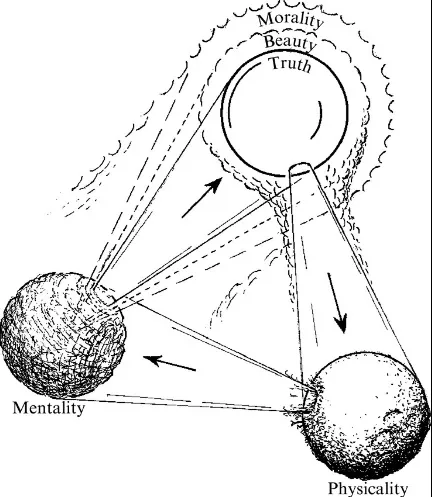
\includegraphics[scale=.35]{a20221106SacredScience107TheHeartoftheMatter-img001.png} 
\caption{Road to Reality}
\end{wrapfigure}

Penrose, in his book \emph{The Road to Reality}, came to the conclusion that there are three worlds, only one of which is amenable to physics. In his earlier works, the diagram that illustrates the Platonic realm of Truth, Beauty, and Morality only included Mathematics. From the Platonic perspective, Mathematics is in between the realm of ideas and the physical world. In his diagram, only Truth is related to the physical world. Penrose has enough self-awareness to recognize that any discussion of beauty or morality has no physical explanation; they make sense only in the mental world.

As for the mental world, he recognizes that any universe that can be observed requires the existence of conscious observers. This requirement places many constraints on the physical world in order for conscious beings to exist at all. This is a version of the Anthropic principle even if no one currently knows all the constraints.

\paragraph{Gross manifestation}

\begin{figure}[t]
\centering
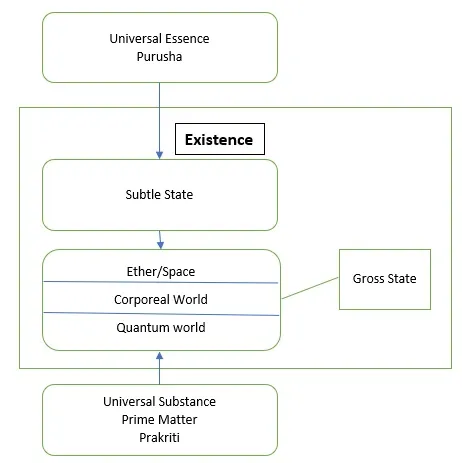
\includegraphics[scale=.5]{a20221106SacredScience107TheHeartoftheMatter-img002.png} 
\caption{World of Things}
\end{figure}

This segues into traditional metaphysics. In this diagram, existence consists of the subtle state and the gross state, which Penrose calls mentality and physicality. In the next installment, the subtle state will be further broken down, but at this point, only the gross state is being described.

\paragraph{Corporeal World}
The Corporeal World is that of our everyday experience, symbolically represented by the elements of Air, Fire, Water, and Earth. This is the world studied by science. Ever since Galileo, at least, science eliminates the sensible experiences of sound, sight, touch, smell, and taste. They belong to the subtle state, or mentality. No fundamental theory of science requires mentality.

As purely physical entities, the science of the corporeal world deals with count, shape or extension, mass, and motion or energy.

\paragraph{Space}
The element Ether is also called Space. It is the bridge between gross and subtle manifestation, since space does not exist in the subtle realm. Although you can pick up a rock, or drink water, you cannot find a piece of space. Nevertheless, space is part of gross manifestation because it is actually formed by matter. In other words, things don't exist in space, but their very existence is space. General relativity demonstrates that a massive distorts the local space around it.

\paragraph{Quantum World}
Physics was motivated to find the smallest unit of matter, which was called the Atom. At first, it seemed successful when the basic elements were organized into the Periodic Table. But as physics kept probing, even more elementary particles were discovered. Ultimately, with quantum theory, there was nothing in particular, just potentiality as described by Schrödinger's Equation. The corporeal world arises when something is measured; what that entails is still not clear to physics. Thus, various interpretations of quantum theory have been proposed to account for it.

Wolfgang Smith has asserted that, with the quantum world, physics has discovered a plane of existence between the traditional Prime Matter and the Corporeal World. That is plausible, since it has characteristics of Prime Matter, yet is physically observable.

\paragraph{Possibilities of manifestation}
If, as physicalists believe, everything that exists arises from the measurement problem, then the existence of things, life, consciousness, and thought must somehow be hidden in Schrödinger's Equation. To date, no one has offered any plausible physical explanation for consciousness or rationality. Yet they are as observable as anything else; actually, the physicist himself illustrates it.

The alternative is to believe in emergent evolution, which is the theory that entirely new properties can arise over the course of time. Obviously, that theory has its own problems, such as explaining the origin of such properties.

In traditional metaphysics, Universal Substance or Prakriti is pure potentiality. All the possibilities of manifestation reside in it. The quantum world is the bridge, then, between Prime Matter and the Corporeal World.

In particular, there is absolutely no physical explanation of the human being. A human being loses and gains matter at every moment, yet the being persists across time. Personal experience demonstrates it. This rules out any multiverse theory. There cannot be a counterpart of a human being in another universe. There is clearly no personal continuity.

\paragraph{Intelligibility}
Now we return to the question of the intelligibility of the world. This requires something that transcends the physical world as Penrose noted. The Essence or Idea of things resides in Purusha. Things are known because the idea of the thing is known. Otherwise, the thing is a mere assemblage of atoms, with the same lack of inherent intelligibility as a mound of windblown sand on the beach.

For those who are time constrained, just listen to the three minute introductions of the three panelists in this video: 

\url{https://youtu.be/W39kfrxOSHg}.

\flrightit{Posted on 2022-11-06 by Cologero}

\begin{center}* * *\end{center}

\begin{footnotesize}\begin{sffamily}

\texttt{veritycacciatrice on 2022-11-07 at 10:10 said: }

“The alternative is to believe in emergent evolution, which is the theory that entirely new properties can arise over the course of time. Obviously, that theory has its own problems, such as explaining the origin of such properties.”

Surely the same properties are always here, appropriate to this world, but the knowledge becomes lost or misinterpreted through time. Humanity cyclically falls like a sack of spuds.

But some mythologists- in describing things that *do* happen- knew eventually civilisation would get back to a certain state of consciousness and technological competence, as it always will, at which time things steeped in dim and boring obscurity, like say… oh I don’t know, the bible for example, suddenly becomes an extraordinarily lucid metaphysic-consciousness handbook almost overnight.

`It’s not just the Big Bang and general relativity that is in trouble, but the foundation of them all.

Gravity is an exhausted and bankrupt concept. A higher, more comprehensive concept is needed. The technologies of gravity have lifted us to a viewpoint that is bigger than gravity.

We need new ideas and new tools such as the Electric Universe model to make sense of the new plasma vistas.’

-Mel Acheson, author of this $>$10min. post from Thunderbolts Project;
\url{https://www.youtube.com/watch?v=dBBJyXwFjWQ}

Note: it is a model, that is, it can be modelled from the lab to cosmic dimensions. Not a theory. 

And on the special bonus plan; `What is Light?’

\url{https://www.youtube.com/watch?v=SZ5ZWbVWMBU}

The question at the end is, what moves? It can only be the consciousness of the observer, which is about as `quantum' as it needs to be.

As an aside, `quantum' is `how much' in Latin.

It’s as if they’re asking us, `How much theory' can you people take until it all blows apart and reality kicks back in.


\hfill

\texttt{Balder on 2022-11-08 at 14:22 said: }

The taichitu explains in a perfectly simple Manner how in manifestation there can never be substance without essence and vice versa.

\hfill

\texttt{Ignatius on 2022-12-26 at 17:06 said: }

It is to be recalled the notion of the `reversal of space and time' as a sign of the times acknowledged in Guénons `Reign of Quantity' and one might notice the apparent significance of the notion of the `event horizon' that has arisen within contemporary mathematical frameworks: as the separation between the environments within and outside an event horizon is marked precisely by the reversal of spatial and temporal components of any trajectory that crosses both environments. As `space' changes into `time', the `event horizon' becomes the trajectory’s `past' and thus cannot be crossed; time changes into space making the `event horizon' a spatial symbol for the separation of `past' and `future' of our perspective. 

The `Reign of Quantity' thus manifests itself in two ways: The discovery (or rather `descent into') a chaotic interim realm between `materia prima' and the corporeal world on the one hand, and the obscure abode of Janus that is the `event horizon' on the other hand; it is to be considered thus not only a spatial symbol of the `end times', but also of `initiation'; a correspondence which should hardly be surprising if one understands the principles underlying the cycle of manifestation.

The truth of this observation is independent of the question whether the mathematical `modes' by which these realities are formulated have any merit whatsoever; the symbolic correspondence is comprehensible inasmuch as they appear in the universal descriptions of the people in this age.

\end{sffamily}\end{footnotesize}